% =====================================================================
% 箱宇宙 -- 日本語版
% 現行版: v0.11-ja(2026-08-22・第167便)。初出は v0.8-ja(2026-07-31・第51便)。
% v0.11-ja(第167便): 英語版 v0.11(改題+感度分析)に等価に追随した。
%   - 改題: 「箱宇宙 — 関係論的トイモデルにおけるプローブ依存の膨張推定」。旧副題が
%     担っていた「意図的に限定したハッブルテンション類似」という限定は失われていない —
%     要旨の免責2文と第VI節に既に在り、そこは不変である。要旨・序論は新題に整合させ、
%     推定量バイアスを先導・ハッブルテンションを動機と比較として後置する順序へ調整した
%     (文の順序と接続の調整のみ。数値・ゲート・図・節構成・主張は1つも動いていない)。
%   - P1-5(外部レビュー第4巡): 第V節に新設 C「比が仮定した減衰則にどれだけ依存するか」 —
%     小表+2段落で「0.92 という値は係数選択の反映」と「プローブ依存自体は一般的」を分離する。
%     出典は tests/exp-p2sens.mjs(committed 出力 tests/out/p2sens-results.json)。
%     同ハーネスは正準構成で committed 図6データを bit 一致で再現してから掃引し(窓 PW1)、
%     本ファイルと英語版へ転記した数値を機械照合する。図の新設はなく、図生成器と
%     その22ゲートは無変更である。
%   - 要旨にその分離を述べる1文を追加した。
% v0.10-ja(第161便): 外部レビュー第4巡対応を英語版 v0.10 と同時反映 — 文言と書誌のみで、
%   数値・ゲート・図・主張は1つも動いていない。
%   - P1-3: 第VI節のハッブルテンション記述が Planck 対 SH0ES の単純な2値対立に
%     読めないよう、JWST 期の複数の距離梯子解析に幅がある旨を2文加え、
%     Freedman et al. (2024) を新規に、既収載の Riess et al. (2024) と併せて引いた。
%     比 0.923 / 0.921 と Dκ 較正は不変。
%   - M-2: 序論に「解決提案ではない」旨の再強調1文、結論部に a→∞ でプローブ比が
%     0 へ収束する挙動は実宇宙に適用できない旨の強調1文(既存の免責・否定的主張と
%     重複しない表現)。
% v0.9-ja(第156便): 外部レビュー第3巡対応を英語版と同時反映 — Code and data
%   availability を現在形に(未来形プレースホルダを本文から削除・TODO(release) は
%   投稿時挿入用にコメントとして維持)/ 要旨の免責を2文へ圧縮(意味は不変)/
%   所属を論文1様式へ統一 / 版番号 v0.8 → v0.9。数値・ゲート・図・主張は不変。
% 英語版 dfm-paper2.tex v0.11 の日本語訳。国内読者向け。
% 学術的な正本(version of record)は英語版であり、本訳と英語版に
% 相違がある場合は英語版が優先する。数値・数式・主張は英語版 v0.11 と同一。
% v0.8-ja(第51便): 外部査読(投稿前)対応の Major revision を英語版と同時反映 —
%   新設 §II「モデルと数値手法」/ 「全数値主張」の範囲限定と claims.sync の位置づけ明確化 /
%   ハッブルテンション比較を Abstract から Discussion へ縮小移設+2024年文献 /
%   dt・光線本数の収束実測 / 暗い天体の節を付録Aへ / Code and data availability 新設 /
%   Abstract 短縮・謝辞の書き直し・検証表の組み替え。
% v0.7-ja 以前の履歴は git を参照。
% Build: lualatex dfm-paper2-ja.tex (2回) — luatexja / HaranoAji フォント
% =====================================================================
\documentclass[a4paper,10pt,twocolumn]{ltjsarticle}

\usepackage{luatexja-fontspec}
\usepackage[haranoaji]{luatexja-preset}
\usepackage{amsmath,amssymb}
\usepackage{bm}
\usepackage{graphicx}
\graphicspath{{figures/}}
\usepackage{booktabs}
\usepackage{array}
\usepackage{tabularx}   % 第143便(P0-3): 検証対応表を段幅内で折り返す
\newcolumntype{Y}{>{\raggedright\arraybackslash}X}
\usepackage{hyperref}
\hypersetup{pdftitle={箱宇宙 --- 関係論的トイモデルにおけるプローブ依存の膨張推定},
  pdfauthor={今村哲矢 (Tetsuya Imamura)}}

% 第167便: 表題は本論文が実際に測っている対象(プローブ依存の膨張推定)を名指す形へ
% 短縮した。旧副題が担っていた限定 —「類似」であって解決の提案ではない — は
% 要旨の免責2文と第\ref{sec:discussion}節に既に在り、表題から外しても弱まらない。
% 改行位置は明示する(自動折り返しだと2行目が「推定」だけの孤立語になる)。
\title{箱宇宙 --- 関係論的トイモデルにおける\\
  プローブ依存の膨張推定\\
  {\large (The Box Universe: Probe-Dependent Expansion Estimates\\
  in a Relational Toy Model)}}
\author{今村 哲矢(Tetsuya Imamura)\\
  {\small 独立研究者(Independent Researcher, Tokyo, Japan)}}
\date{2026-07-31(ドラフト v0.8-ja)/ 2026-08-21 改訂(ドラフト v0.9-ja)/
  2026-08-22 改訂(ドラフト v0.10-ja・v0.11-ja)}

\begin{document}
\maketitle

\begin{abstract}
先行論文で導入した2次元の関係論的トイモデル「決定力場モデル(DFM)」を、
\textbf{箱宇宙}近似---有限領域の外側すべてを単一の単純化された背景で置き換える---の
導入によって拡張する。
% 第167便: 要旨は新題が名指す測定結果を先導させる。文の順序と接続だけの調整であり、
% 免責2文・数値・節構成は不変である。
中心結果は\textbf{プローブ依存の膨張推定}---誤指定した減衰則のもとでの推定量バイアス
---である: 同じ箱に適用した幾何プローブと
速度減衰プローブが返す膨張率の比は解析係数
$H_w/H_{\mathrm{geo}}=2D\kappa\,d_P\,a^{-d_P}$ になる。速度観測者が、指数則の生成した
データに FLRW の $w/c\propto1/a$ を当てはめるからである。実測の比は解析係数と
$5.3\times10^{-4}$ まで一致する。
減衰係数・観測時期・推定量のビニングを掃引すると、比は選んだ係数に比例し
(較正値 $0.92$ はその選択の言い換えである)、食い違いそのものは全構成で残る。
箱はまた古典的な関係論の問いを計算可能にする: 箱全体の一様並進は
指定した内部観測量を bit 一致のまま変えず、回転と膨張は、解析的中心極限 $g(0)=1/2$ に
漸近する実測の動径利得を通じて内部に結合する。膨張は、規定された運動学・波長の意味論・
解かれる動力学という機械検証された3層に分離される。
プローブの結果は\textbf{プローブに依存するハッブル定数の推定への
限定された類似}を与える: ある推定量が別の推定量と食い違うのは、誤った減衰則を仮定して
いるからでありうる、ということである。
本論文は宇宙論的なハッブルテンションのモデルでもなければ、その解決の提案でもない。
シミュレーション由来の中心的な数値主張はすべて、継続的インテグレーションで走る
自動検証ゲートに紐づいている。
\end{abstract}

% ---------------------------------------------------------------------
\section{はじめに}
\label{sec:intro}

先行論文~\cite{DFM1}では決定力場モデル(DFM)を導入した。これは空間が純粋に関係論的である
教育用トイモデルであり、各点のあらゆる力学的性質はスカラーの\textbf{決定力場} $W$ を
通じて周囲の質量から定まり、慣性・重力・時計の進み・光の伝播はすべてそこから読み出される。
先行論文は実質的に無限の背景の上で、局所的な帰結---フレーム引きずり・回転曲線・時計・
レンズ効果---を調べた。

本論文は近似の反対側の端を調べる。「宇宙の残り全部」を意図的に単一の単純化された
対象で置き換えたとき、何が起こるか。この対象を\textbf{箱}と呼ぶ。
箱宇宙は新しい公理ではない。選んだ半径の外側の決定力源を、一様背景項 $D_0$、
スケール因子 $a(t)$ を伴う箱決定力 $D$、および任意で一様重力ベクトルに要約する、
という宣言である。トイモデルが問える宇宙論的な問い---何が膨張するのか。何が共動なのか。
赤方偏移とは何を意味するのか。膨張は規定するだけでなく\textbf{解ける}のか---は
すべて箱についての問いになり、モデルが小さく決定論的であるおかげで、それぞれの答えを
機械検証できる。

我々の立場は先行論文から変わらない。DFM は教育用の\textbf{計算的思考実験}であって、
自然についての提案ではない(第\ref{sec:negative}節)。
% 第167便: 第161便(M-2)の同じ2文を、新題が求める順序 — まず本論文が提示するもの、
% その後にハッブルテンションを動機・比較として — に並べ替えた。接続語以外の文言は不変。
本論文が提示するのは、そして新題が名指すのは、率の推定における1つの\textbf{失敗様式}
---推定者が仮定した減衰則をそのまま引き継いでしまうこと---を手のひらに載る
大きさにする機構である。
% 第161便(M-2): 強調の1文。否定的主張3・6や要旨の免責と重複しない表現にしてある。
この立場から従うことを1つ、末尾の否定的主張に委ねずに先に述べておく: 本論文は
ハッブルテンションの解決案を何ひとつ提示しないし、読者はここでそれを見出さない。
いま述べた機構は、実在の食い違いに対する説明の提案とは別種の対象である。
箱宇宙の面白さは、教科書的な
区別---運動学的膨張と動力学的膨張、座標の後退と測定される赤方偏移、プローブと量---を、
学生がブラウザで切り替えられるほど具体的にし、本論文の中心的な数値を
継続的インテグレーションのスイートが assert していることにある。

本論文の構成は次のとおり。第\ref{sec:methods}節でモデル・数値手法・誤差の分類を定義する。
第\ref{sec:box}節で箱を定義し、内部から何が検知でき何ができないかを確立する。
第\ref{sec:layers}節で膨張を3つの検証済みの層に分離する。
第\ref{sec:probe}節が主結果---プローブ依存の膨張推定---であり、末尾で較正値と機構を
分離する感度分析を行う。
第\ref{sec:discussion}節で推定量バイアスとしての読みと、意図的に限定した
ハッブルテンションとの類似を論じる。第\ref{sec:negative}節で主張の一部をなす6つの
否定的主張を述べ、第\ref{sec:repro}節で中心主張を検証ゲートに対応づけ、コードとデータの
入手可能性を記す。付録\ref{app:dark}では同じ機構をモデルの光学的に暗い重力体に適用する。

% ---------------------------------------------------------------------
\section{モデルと数値手法}
\label{sec:methods}

\subsection{場・力・時計・光}

DFM は2次元の粒子モデルである。位置 $\bm r_j$ の質点 $m_j$ はスカラーの
\textbf{決定力場}
\begin{equation}
  W(\bm r)=D_0+W_B+\sum_j \frac{m_j}{\sqrt{|\bm r-\bm r_j|^2+\epsilon^2}}
  \label{eq:W}
\end{equation}
の源となる。$\epsilon$ は Plummer 軟化長、$D_0$ は一様背景、$W_B$ は
第\ref{sec:box}節で定義する箱項である。重力は同じ軟化を持つニュートン的な対引力である。
スピンする質量は局所の\textbf{決定フレーム}を引きずり(強さは大域結合
$k_{\mathrm{Frame}}\in[0,1]$)、動く背景は同じチャネルで自由粒子を輸送する
(モデルのマッハ的セクター)。時計の進みと光の伝播はどちらも単一の無次元ポテンシャル
$\psi=W\kappa$ から読まれる: 固有時は $d\tau/dt=e^{-\psi}$ で進み、局所光速は
$c_{\mathrm{loc}}=c_0\,e^{-2\psi}$、有効屈折率は $n_{\mathrm{eff}}=e^{2\psi}$ である。
$W$・$D$・$D_0$ は(任意の)シミュレーション質量単位/長さの次元を持ち、時空係数
$\kappa$(実装のパラメータ \texttt{kappaT})はその逆数(質量あたりの長さ)を持つ。
これで $\psi$ が無次元になる。$\kappa$ は $G/c^2$ と同じ次元の量であり、一般相対論の
アインシュタインの重力定数 $\kappa=8\pi G/c^4$ とは記号を共有するだけの\textbf{別の量}
である。長さ・時間・速さはすべて内部単位で、
以下の主張はどれもその物理較正に依存しない。本論文で使う任意セクター:
スピン/熱を持つ粒子間の圧力様の対斥力(遠方force $F\propto d^{\,1-2q}$。
第\ref{sec:layers}節)、散逸的な接触(法線減衰と並進→スピン摩擦)、伝導、放射冷却。
これらは有効と明記した箇所以外ではすべて切ってある。

\subsection{積分と状態}

運動方程式は固定刻み $\Delta t=0.016$ の1次半陰的(シンプレクティック)オイラー法で
積分する。時間対称な leapfrog(KDK)も選択でき、可逆性そのものを試験する箇所でのみ使う。
状態はすべて倍精度である。発散防止の安全クランプ(速度・スピン・膨張率の上限)は
帳簿が発動回数を数え、保存則を主張するすべての構成で\textbf{発動0回}を検証ゲートが
assert する。運動量・角運動量・エネルギーの帳簿は明示的なリザーバ台帳に対して閉じ、
保存則型のゲートは「小さなドリフト」ではなく閉じた総和を assert する。

\subsection{測定量}

本論文で使う観測量は一度だけ定義し、全体で再利用する。窓 $[t_1,t_2]$ の
\textbf{幾何膨張率}は $H_{\mathrm{geo}}=\Delta\ln a/\Delta t$。
\textbf{速度減衰推定}は $H_w=-\Delta\ln R/\Delta t$($R=w/c_{\mathrm{loc}}$。$w$ は
規定 Hubble 流に対する特異速度)。窓平均は常に窓とともに引用し、$t=0$ 基準の
\textbf{累積}推定量と\textbf{局所窓}推定量は現れる場所ごとに区別する。自由な箱の
\textbf{実効スケール因子}は壁質量から測る
$a_{\mathrm{eff}}=\langle r_{\mathrm{wall}}\rangle/\langle r_{\mathrm{wall}}\rangle_0$。
光線実験の観測面光束と捕捉率は付録\ref{app:dark}で定義する。

\subsection{誤差の分類と検証の独立性}
\label{sec:taxonomy}

機械検証された各主張は、コード上で主張の隣に宣言された5種類の検証形態のいずれかを持つ:
\textbf{解析一致}(閉形式との一致)・\textbf{保存恒等式}(帳簿の閉じた総和)・
\textbf{意味論回帰}(定義・表示規則)・\textbf{固定seed実測}(決定論的単一走行)・
\textbf{多seed統計}(シード間の広がり。$\pm$ はシード間標準偏差)。
この機構には2つの誠実性の注記が付く。第一に、図データの多くはシミュレータ自身を
駆動して生成される。これは図と実装の同期を保証するが、実装が正しいことの独立証明では
ない。解析一致ゲートはエンジンの外(テストハーネス側)で評価した短い閉形式と比較し、
保存恒等式は解析予測から独立である。第二に、いくつかのゲート許容値は最初の実測の
\textbf{後に}設定された。それらは記録値を固定する回帰基準であって盲検の予測ではなく、
固定seed型と分類されている。

離散化は中心結果について直接調べた: 時間刻みを半分・さらに半分にすると、
第\ref{sec:probe}節のプローブ比誤差は $5.3\times10^{-4}$($\Delta t=0.016$)→
$2.7\times10^{-4}$($0.008$)→ $1.1\times10^{-4}$($0.004$)と単調に減り、1次積分器と
整合する。引用している許容値 $10^{-2}$ は、本番刻みでの実測誤差の2桁上にある。

% ---------------------------------------------------------------------
\section{近似としての箱}
\label{sec:box}

\subsection{意味論}
\label{sec:semantics}

箱宇宙は6つの意味論的コミットメントで定義される(正準な記述はプロジェクトの
箱宇宙文書 §12):
(1) 有限領域の外側では、決定力源はシミュレートされず要約される。
(2) 要約は、一様背景 $D_0$、スケール因子 $a(t)$ が運ぶ箱項 $W_B=D\,a^{-d_P}$、
および任意の一様重力ベクトルからなる---概念上、これらはすべて\textbf{箱のパラメータ}である。
(3) 内部の物理は不変である: 同じ公理が、どこから来たものであれ合計の場 $W$ を読む。
(4) 箱は\textbf{規定}(調律された $a(t)$)でも\textbf{自由}(通常の質量でできた壁の運動が
$a(t)$ を解く)でもよい。
(5) 共動座標と波長の意味論はその上に載る定義であり、それぞれ固有の検証を持つ。
(6) 以上のどれも実宇宙についての主張を含意しない。

\subsection{内部から検知できないもの}

モデルのすべての公理は相対配置のみに依存する(式(\ref{eq:W})と対力則は座標差の関数で
ある)から、箱全体の一様並進は力学の対称性である。検証スイートはさらに、追跡している
観測量(位置・速度・スピン・時計)について、実装された内部進化がブーストされた箱の下で
bit 一致であることを機械精度で assert している。したがって「厳密な検知不能性」の主張は
実装の指定観測量についてのものであり、一般化は解析的な対称性の議論が担う。
回転と膨張は異なる: これらは決定フレームを通じて、測定される\textbf{利得}
$g(r)$ とともに入り込む。壁質量の一様リングでは、源についての方向射影位置の
解析平均が
\begin{equation}
  \bigl\langle \hat n\,(\hat n\cdot\bm r)\bigr\rangle=\tfrac{1}{2}\bm r
  \label{eq:gain}
\end{equation}
を与えるので、内部中心は壁の回転・膨張に利得 $g(0)=1/2$ で結合する。中心の値は
解析極限であり(測定推定量は中心で $0/0$ になる)、半径スキャンの最内点 $r=20$ の実測は
$g=0.5002$ --- スキャン全体が解析曲線と一致することが極限を支える(ゲート V23a/V24a)。
これは古典的な関係論の主張~\cite{Mach1893,BarbourBertotti1982}のトイモデル版
---類似であって、同一の理論的結論ではない---である:
絶対的な一様運動は無意味だが、「それ以外の全部」の絶対回転・絶対膨張は、それが引きずる
フレームを通じて内部から観測可能である。
図\ref{fig:hierarchy}に構成の模式を、図\ref{fig:gain}に実測利得と解析曲線の比較を示す。

\begin{figure*}[t]
  \centering
  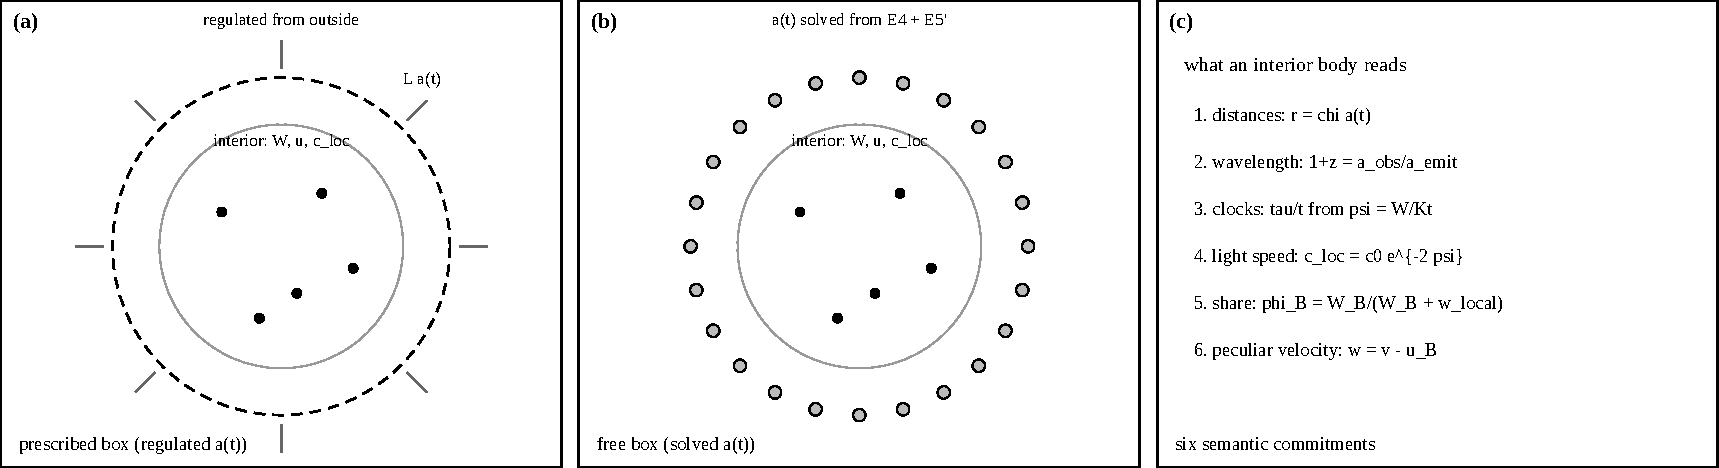
\includegraphics[width=\textwidth]{p2fig1.pdf}
  \caption{箱の階層。(a) \textbf{規定}の箱: 壁は外から調律される名目半径 $L\,a(t)$ で、
  要約された背景は場を通してのみ内部に入る。(b) \textbf{自由}な箱: 壁は普通の質点で
  できており、$a(t)$ は与えられるのではなく解かれる(第\ref{sec:layers}節)。
  (c) 内部のあらゆる物体が読む量と、第\ref{sec:semantics}節の意味論6項目。
  模式図でありシミュレーションデータは含まない。(c) は時計ポテンシャルを旧表記
  $\psi=W/K_t$($K_t=1/\kappa$)で書いている。生成: \texttt{tools/gen-figures2.mjs}。}
  \label{fig:hierarchy}
\end{figure*}

\begin{figure}[t]
  \centering
  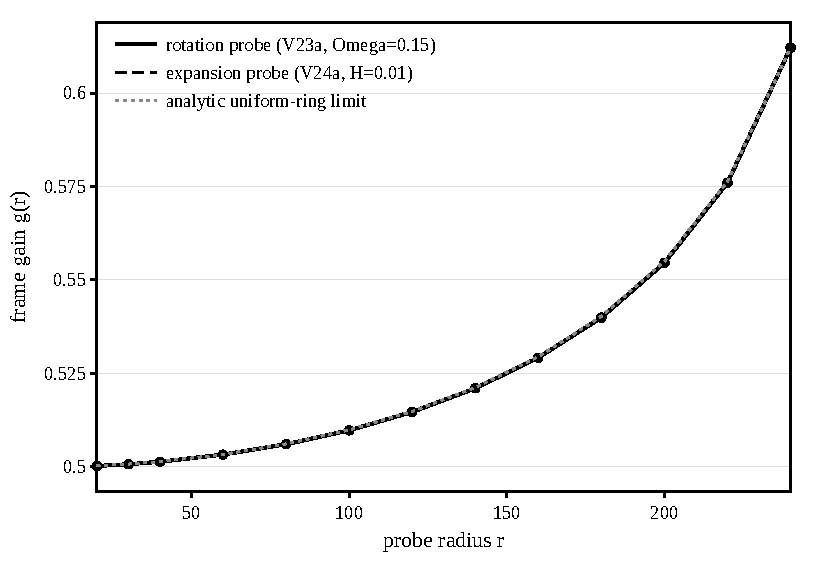
\includegraphics[width=\linewidth]{p2fig2.pdf}
  \caption{質点リング壁($N=96$、$m=20$、$R=260$、$\epsilon=4$、$k_{\mathrm{Frame}}=1$、
  $G=0$)のフレーム利得 $g(r)$。測定は検証ゲート V23a(回転・$\Omega=0.15$)と
  V24a(膨張・$H=0.01$)の構成をそのまま半径スキャンへ拡張したもので、各半径に方位4点の
  プローブを置く。回転と膨張の実測が重なるのは当然で、両者は同じ加重平均を通って結合する。
  灰色は連続一様リング極限の解析値 $g(r)=(R/r)\,I_c/I_0$
  ($I_c=\oint\cos\theta\,\mathrm d\theta/\sqrt{d(\theta)^2+\epsilon^2}$、
  $I_0=\oint \mathrm d\theta/\sqrt{d(\theta)^2+\epsilon^2}$。$d(\theta)$ はプローブ点から
  方位 $\theta$ のリング要素までの距離)であり、その $r\to0$ 極限が
  式(\ref{eq:gain})である。実測 $g(20)=0.5002$(両プローブ)、スキャン全域での
  解析曲線からのずれは最大 $0.07\%$。}
  \label{fig:gain}
\end{figure}

% ---------------------------------------------------------------------
\section{膨張の3つの層}
\label{sec:layers}

\subsection{第1層: 規定された運動学}

調律された $a(t)$ のもとで、箱は動力学なしの FLRW 型の帳簿を提供する。
完全共動粒子の共動座標 $\chi=r/a$ は検証ランで $1.5\times10^{-5}$ まで保存される
(V24b)。束縛系は箱に部分的にしか追随しない: 軌道スケーリングの実測
$d\propto a^{n_{\mathrm{eff}}}$ の指数は、軌道位置での箱の決定力の持ち分
$\varphi_B$ とともに増える(V25: 正味指数は $\varphi_B\to1$ で $1.61$、
$\varphi_B\to0$ で $0.00$)。教科書の
「束縛系は膨張しない」は、測定されたダイヤルの $\varphi_B\to0$ の端として得られる
(図\ref{fig:phib})。

\begin{figure}[t]
  \centering
  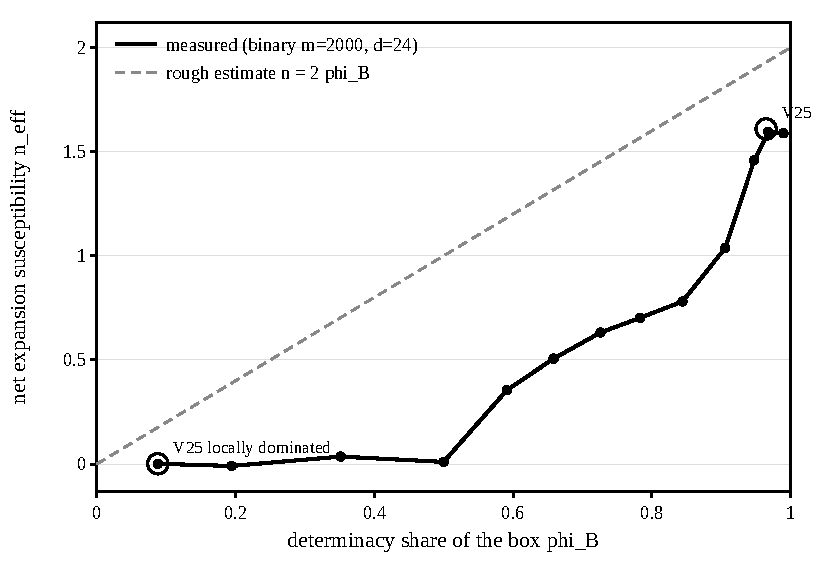
\includegraphics[width=\linewidth]{p2fig3.pdf}
  \caption{膨張への追随はスイッチではなくダイヤルである。束縛連星の正味膨張感受率
  $n_{\mathrm{eff}}$($d\propto a^{n}$)を、箱の決定力の持ち分
  $\varphi_B=W_B/(W_B+w_{\mathrm{local}})$ に対して示す。測定は V25 の構成
  (規定 $H=0.004$ の箱を $a=1.2$ まで走らせ、$H=0$ 統制との差を取って内部散逸を相殺)。
  スキャンは連星($m=2000$、$d=24$)を固定し、箱の決定力 $D$ のみを振る。丸印は V25 の
  2つのゲート点で、箱支配の連星($\varphi_B=0.965$、$n=1.61$)と局所支配の連星
  ($\varphi_B=0.088$、$n=0.00$)。破線はエネルギー励起の粗見積 $n=2\varphi_B$ で、
  実測がこれに近づくのは箱支配の端だけである。}
  \label{fig:phib}
\end{figure}

\subsection{第2層: 波長の意味論}

箱の中の赤方偏移は\textbf{意味論的}な規則である: 放たれた光は波長比
$1+z=a_{\mathrm{obs}}/a_{\mathrm{emit}}$ を保つ。スイートは同じランの異なる時期に
2つの共動源 A・B から光を放ち、第3の共動観測者 C での到着をほぼ同時($\Delta t=0.016$)に検査する
(ゲート \texttt{box.photon-abc}、帳簿の閉じ残りは $10^{-9}$ 未満。図\ref{fig:abc})。

\begin{figure}[t]
  \centering
  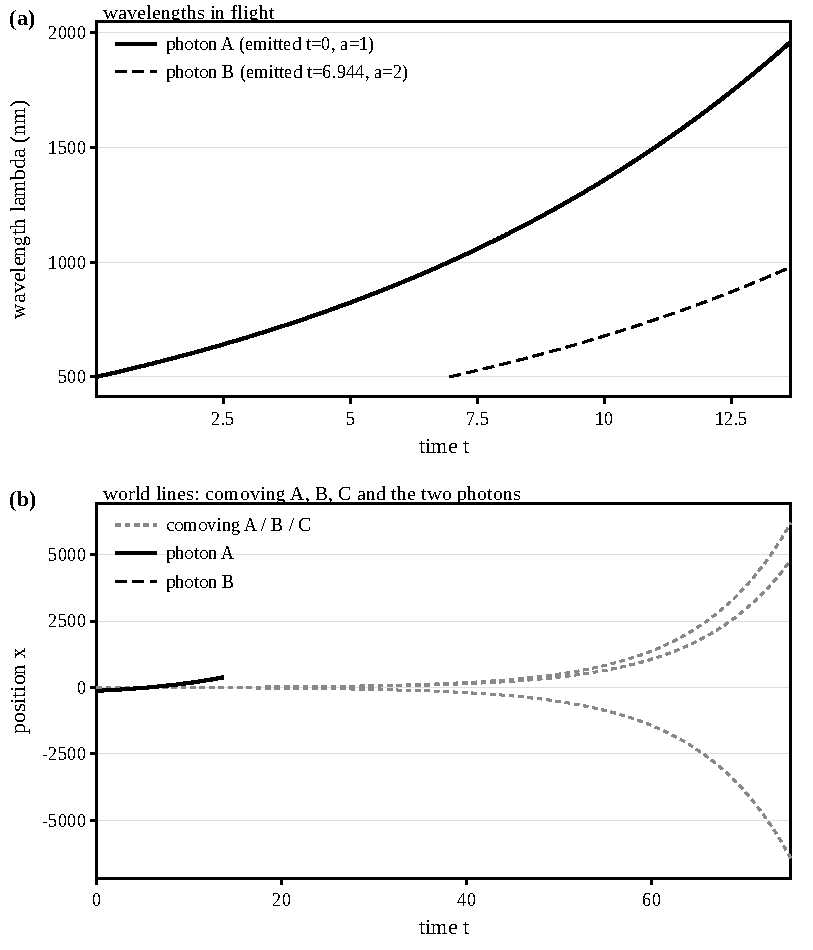
\includegraphics[width=\linewidth]{p2fig4.pdf}
  \caption{A/B/C 思考実験の実行(プリセット \texttt{boxredshift}、$H=0.1$、$d_P=1$ — v1.39 の
  一律光速規約 c₀=30 への再パラメータ化。以前に示した run の厳密な力学的相似〔時間 ÷5・率 ×5〕で、
  赤方偏移はすべて相似不変)。
  (a) 飛行中の波長 $\lambda(t)=\lambda_E\,a(t)/a_E$。A は $t=0$($a=1$)に $500$\,nm を、
  B は $t=6.944$($a=2$)に $500$\,nm を放ち、どちらも $t\approx13.7$ に C で観測される
  ($1964$\,nm・$z=2.927$ と $979$\,nm・$z=0.958$)。(b) 世界線。B の放出以降、2つの光子は
  同じ経路をたどるので、異なる時期に放たれた光が異なる赤方偏移を担って同時に届く。
  帳簿 $|\lambda_{\mathrm{obs}}/\lambda_{\mathrm{emit}}-
  a_{\mathrm{obs}}/a_{\mathrm{emit}}|$ は機械ゼロまで閉じる---これが否定的主張2の内容で、
  導出ではなく規則だということである。}
  \label{fig:abc}
\end{figure}これは運動学の上に載せた定義であって光子力学からの
導出ではない(本論文の否定的主張2)。その価値は、観測される整合関係---超新星の時間伸長
$\propto(1+z)$~\cite{Leibundgut1996,Goldhaber2001} と
$T_{\mathrm{CMB}}(z)=T_0(1+z)$~\cite{Fixsen2009,Noterdaeme2011}---に現れるのと同じ
スケール因子依存性を\textbf{符号化する}ことにある(それらの観測量そのものはここでは
シミュレートしない)。学生は、そうした関係のどこまでが意味論でどこからが物理かを
正確に見られる。

\subsection{第3層: 解かれる動力学 --- 自由な箱}

調律された箱を64個の自由な壁質量で置き換えると、$a(t)$ は出力になる。
駆動するのはスピンする壁質量間の\textbf{圧力様の対斥力}である --- 熱力学的な状態方程式や
応力エネルギーの圧力ではない。「圧力」の語は本論文全体でこの緩い・機構水準の意味で使う。
斥力があるとき、実効スケール因子の実測は $a_{\mathrm{eff}}=2.18$ まで加速する。
遠方の対斥力は $F\propto d^{\,1-2q}$ でスケールし、本プリセットは $q=1$ を使うため
$1/d$ 減衰---重力より遅く、大分離で勝つ(DFM 既定の $q=2$ では $1/d^{3}$ となり勝てない)。
$2.18$ という値はこの離散リング構成($q=1$・$k_{\mathrm{Rep}}=0.5$・等質量壁64個)の
性質であって普遍的な数ではない --- 用量反応はアプリ内 A/B で確認でき、
$G\times k_{\mathrm{Rep}}$ の4象限スキャンが加速の源を斥力そのものに固定する(重力の
減速寄与は $a_{\mathrm{eff}}$ で $-0.013$)。斥力を除くと
($k_{\mathrm{Rep}}=0$)同じ箱は $a_{\mathrm{eff}}\approx1.005$ で頭打ちになり
再収縮する。このランは完全な閉鎖系である: リザーバ帳簿は恒等的にゼロで、
運動量・角運動量のドリフトは $4\times10^{-8}$ 未満(ゲート \texttt{freebox.*})。
これはフリードマン宇宙論の精神における機構のデモ---引力は減速させ、圧力様の斥力は
加速させうる---であり、フリードマン方程式の再現主張ではない(否定的主張5)。
図\ref{fig:freebox}。

\begin{figure}[t]
  \centering
  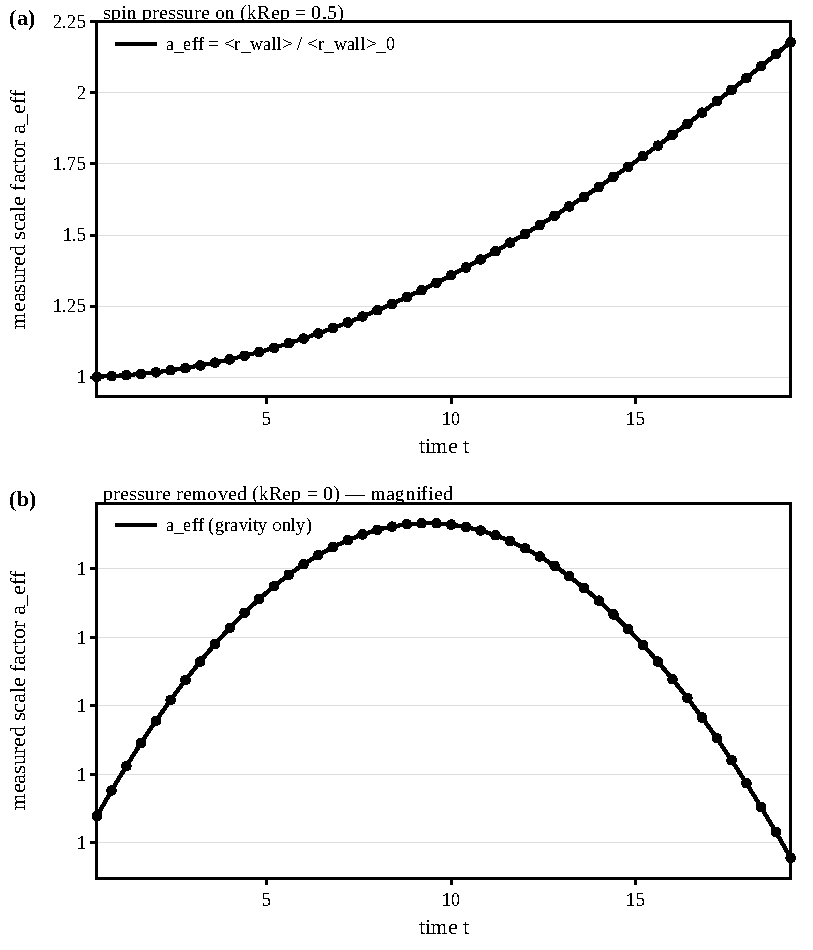
\includegraphics[width=\linewidth]{p2fig5.pdf}
  \caption{自由な箱は自分の膨張則を解く(プリセット \texttt{freebox}、64個の自由な壁質量、
  $1200$步=$t=19.2$)。描かれている
  $a_{\mathrm{eff}}=\langle r_{\mathrm{wall}}\rangle/\langle r_{\mathrm{wall}}\rangle_0$ は
  規定値ではなく壁から測った実測値である。(a) 対斥力あり($k_{\mathrm{Rep}}=0.5$)では
  $a_{\mathrm{eff}}=2.1795$ に達し、しかも\textbf{加速}する($H_{\mathrm{eff}}$ が
  $3.18\times10^{-2}$ から $5.14\times10^{-2}$ へ)。(b) 同じ箱から斥力を除いた場合の拡大図:
  重力だけの宇宙は $t=9.2$ の $a_{\mathrm{eff}}=1.0047$ で頭打ちになり再収縮する
  ($H_{\mathrm{eff}}$ が $+4.42\times10^{-4}\to-5.28\times10^{-4}$ と符号反転)。
  どちらのランでもリザーバ帳簿は恒等的にゼロである(ゲート \texttt{freebox.*})。}
  \label{fig:freebox}
\end{figure}

\subsection{補: 可逆な箱の中の時間の矢}

leapfrog 積分器のもとで、この力学は本有限テストの範囲で RMS $1.3\times10^{-3}$ まで
操作的に可逆である: 全速度・全スピンを反転するとその精度で初期状態へ戻る。
散逸チャネルを1つ入れると($\mu_F=0.3$)戻りは壊れる(RMS $10.8$)。既定の半陰的積分器は
決定論的だが、やはり巻き戻せない(RMS $0.92$ --- $709$倍の劣化)。この実験が分離するのは
決定論と可逆性である: 散逸は矢の一因であり、時間反転対称でない離散化は、それとは別の
純粋に数値的な矢を作る(ゲート \texttt{echo.*})。本節は意図的に簡潔に留める。
詳しい扱いは今後の課題である。

% ---------------------------------------------------------------------
\section{プローブ依存の膨張推定}
\label{sec:probe}

\subsection{ハッブル反摩擦と比の基準}

DFM では、自由粒子の特異速度 $w$ は、箱が膨張していてもモデルの絶対的な帳簿では
保存される(実測ドリフト $<10^{-3}$。ゲート V27/V28)。減衰するのは\textbf{比}
$R=w/c_{\mathrm{loc}}$ である: 箱の決定力が希釈されると局所光速が上がる。
$c_{\mathrm{loc}}=c_0\,e^{-2\psi}$($\psi=W_B\kappa$)であり、
\begin{equation}
  R(a)=\exp\!\bigl[-2D\kappa\bigl(1-a^{-d_P}\bigr)\bigr]
  \label{eq:R}
\end{equation}
が $a=2$ で $2.5\times10^{-4}$ まで検証されている(V28)。光---内部観測者が使える操作的基準の一つ---で測るかぎり、自由運動は FLRW の $w\propto1/a$ 摩擦~\cite{Peacock1999}と同じ向きに\textbf{減衰して
見える}。ただし関数形は異なる。

\subsection{2つのプローブ、1つの箱}
\label{sec:v29}

いま、2人の観測者が同じ箱の膨張率を測るとする。\textbf{幾何}観測者は共動構造を
追跡して $H_{\mathrm{geo}}=\Delta\ln a/\Delta t$ を報告する。\textbf{速度}観測者は
FLRW 運動学($w/c\propto1/a$)を仮定し、$R$ の減衰の実測から膨張率を推定する:
$H_w=-\Delta\ln R/\Delta t$。式(\ref{eq:R})から
\begin{equation}
  \frac{H_w}{H_{\mathrm{geo}}}=2D\kappa\,d_P\,a^{-d_P}
  \label{eq:ratio}
\end{equation}
であり、これは時期 $a$ と箱の較正 $D\kappa$ に依存する。2つのプローブは食い違う。
どちらかが間違っているからではなく、モデルの減衰則が第2の観測者が仮定した FLRW の
それではないからである。

検証ゲート V29 は1つのランで両プローブを3窓($a\colon1\to1.5\to2\to3$、$d_P=1$)
にわたり測定し、測定された比を式(\ref{eq:ratio})の対数窓平均と比較する。相対誤差の
最大は許容値 $10^{-2}$ に対して $5.3\times10^{-4}$、$w$ の保存は
$4.8\times10^{-4}$ である。図\ref{fig:probeH} の背後にある24窓の拡張スキャンの
最大相対偏差は $6.2\times10^{-3}$ であり、両者は別物の精度だが、いずれも事前宣言の
許容値 $10^{-2}$ を満たす。誤差は離散化が支配し、刻みとともに収束する
(第\ref{sec:taxonomy}節)。
図\ref{fig:probeH}は、このゲートを比較実験設計 4-66 に従って
$a\times(D\kappa)$ のスキャンへ拡張したものである。この比較実験は独立実験スクリプトとして
実装済みで、その実測記録は事前宣言の判定4基準(指数系列の精度・対照の恒等性・
曲線分離 $>10\sigma$・V29 回帰ゲート)をすべて満たし、出力は図6のデータ源を兼ねる。

\begin{figure}[t]
  \centering
  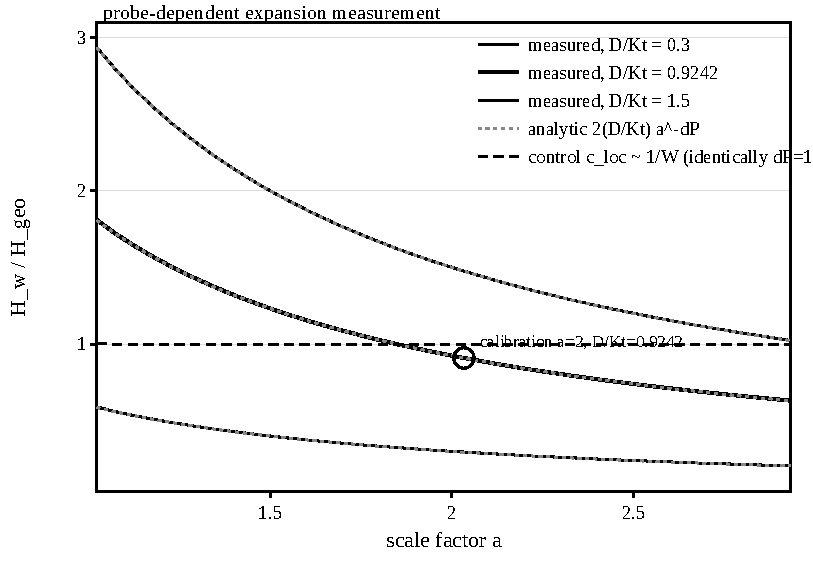
\includegraphics[width=\linewidth]{p2fig6.pdf}
  \caption{プローブ依存の膨張測定。実測 $H_w/H_{\mathrm{geo}}$(黒)と解析式(\ref{eq:ratio})
  (灰)を3つの箱較正について示す。規定の指数膨張箱の中の自由粒子1個から測定
  ($\kappa=1/300$、$c_0=60$、$H_0=0.01$、$d_P=1$、$a\colon1\to3$ を24窓)。各実測窓の横軸は
  「点値が窓平均に一致する $a$」に置いてある。解析曲線からのずれは相対で最大
  $6.2\times10^{-3}$、特異速度 $w$ の保存は $4.8\times10^{-4}$。破線は
  モデル内対照で、同じ実測 $w$ を厳密反比例の光速則($c_{\mathrm{loc}}\propto1/W$)に対して
  読み直すと $H_w/H_{\mathrm{geo}}\equiv d_P=1$ となり、プローブ依存が消える。丸印は較正点
  $a=2$、$D\kappa=0.9242$ で、ここでは食い違いが恒等的に $D\kappa$ に等しい。この点における
  2つの光速則の差 $0.076$ は達成された測定精度の $21$ 倍であり、どちらの法則かは
  モデルの内側から観測可能である。図中のラベルは較正を旧表記 $D/K_t$($K_t=1/\kappa$)で
  書いており、数値としては $D/K_t=D\kappa$ である。}
  \label{fig:probeH}
\end{figure}

関数形が効果の内容のすべてである。もしモデルの光速則を厳密反比例
$c_{\mathrm{loc}}\propto1/W$ に置き換えると、$R\propto a^{-d_P}$ が
厳密に成り立ち、両プローブは恒等的に一致し($H_w/H_{\mathrm{geo}}\equiv d_P$)、
プローブ依存性は消える。2つの法則のどちらを選ぶかは\textbf{モデルの内側から観測可能}
である。これが教育的な要点である: 測定の不一致に見えるものは、自然(ここでは公理系)が
実際にどの減衰則を使っているかについての主張でありうる。

1点を正確に述べ直す(旧稿の誤りを外部レビューが指摘し訂正した): $d_P=1$ では比
$\rho(a)=2D\kappa/a$ は単調に低下するが、プローブの\textbf{食い違い} $|\rho-1|$ は
単調ではない。プローブが厳密に一致するのは $a=2D\kappa\approx1.85$ のただ1回であり、
食い違いはそこまで縮み、その後は再び拡大する。
後期の振る舞いには名前を付けておく価値がある。宇宙論へ移せないのがまさにこの部分だから
である: $a\to\infty$ では比 $\rho(a)=2D\kappa/a$ がゼロへ落ちるので、速度プローブは
幾何プローブに比べていくらでも小さい膨張率を報告し、2つの推定量は共通値へ落ち着くのでは
なく際限なく乖離する。この極限は公理に書き込まれた指数型の光速則の性質であり、しかも
箱近似が何かの妥当な要約であることをとうにやめている領域で到達される。
したがってこのモデルが与えるのは「プローブ依存性」であって、「食い違いが早期から後期へ
単調に緩和する」ことではない。後期極限は公理についての言明であって予言ではない。

% ---------------------------------------------------------------------
% 第167便(P1-5): 外部レビュー第4巡は、減衰係数・観測窓・推定量定義を振って
% 「0.92 という値」と「一般に生じるプローブ依存」を、論じるのではなく分離して示すことを
% 求めた。本小節と下の表の数値はすべて tests/out/p2sens-results.json からの機械転記で
% あり、ハーネス tests/exp-p2sens.mjs が本ファイルと英語版を自身の出力と照合する。
% 図の新設はない(図生成器とその22ゲートは無変更)。
\subsection{比が仮定した減衰則にどれだけ依存するか}
\label{sec:p2sens}

較正 $D\kappa=0.9242$ は1つの選択である(第\ref{sec:discussion}節・否定的主張6)。
であれば読者は「結果のどこまでがその選択で、どこからが機構なのか」を問う権利がある。
リポジトリの感度分析ハーネス(\texttt{tests/exp-p2sens.mjs}、記録出力
\texttt{p2sens-results.json})が機械的に答える。
このハーネスは第\ref{sec:v29}節の測定を同じ公理から再実装し、まず正準構成で
図\ref{fig:probeH}の背後にある committed データを\textbf{bit 一致}で再現したうえで、
モデルが固定していない3つ---減衰係数 $D\kappa$、観測する時期の範囲、推定量がその範囲を
どう分割するか---を掃引する。2つのプローブ・推定式・集約規則はどの構成でも同一であり、
変わるのは掃引した量だけである。窓と数値床は実測前に固定した。

\begin{center}
{\footnotesize\setlength{\tabcolsep}{4pt}
% BEGIN p2sens-table(tests/out/p2sens-results.json からの機械転記 —
% 手で編集しないこと。ハーネス tests/exp-p2sens.mjs が全項目を自身の出力と照合する)
\begin{tabular}{lcccccc}
 & \multicolumn{2}{c}{$a\colon1\to\sqrt3$}
 & \multicolumn{2}{c}{$a\colon1\to3$}
 & \multicolumn{2}{c}{$a\colon1\to9$} \\
$D\kappa$ & $\ln a$ & $a$ & $\ln a$ & $a$ & $\ln a$ & $a$ \\
\hline
0.5 & 0.770 & 0.751 & 0.607 & 0.550 & 0.405 & 0.276 \\
0.75 & 1.155 & 1.126 & 0.911 & 0.824 & 0.607 & 0.414 \\
0.9242 & 1.423 & 1.387 & 1.122 & 1.016 & 0.748 & 0.509 \\
1.25 & 1.924 & 1.876 & 1.517 & 1.374 & 1.012 & 0.689 \\
1.5 & 2.309 & 2.251 & 1.821 & 1.649 & 1.214 & 0.826 \\
\end{tabular}
% END p2sens-table
}
\end{center}

\noindent
表は掃引した30構成すべての $H_w/H_{\mathrm{geo}}$ である: 5つの減衰係数(行)、
3つの観測時期の範囲(列群。中央が図\ref{fig:probeH}の範囲)、そして各範囲を24の
部分窓へ分ける2通りのビニング---$\ln a$ について等間隔(正準の取り方)と $a$ について
等間隔。各項目は24個の部分窓の比の平均である。

ここから3つの読みが出る。要点は、この3つが\textbf{種類として異なる}ことである。
第1に、範囲とビニングを固定すれば比は $D\kappa$ に $1.2\times10^{-3}$ の精度で比例する:
$0.92$ という数は較正の言い換えであって、機構の出力ではない。
第2に、残る2つの選択は、較正が合わせに行った $7.6\%$ の差と同程度に比を動かす ---
$D\kappa=0.9242$ で、同じ走行を $\ln a$ 等間隔から $a$ 等間隔へビニングし直すだけで比は
$9.5\%$ ずれ、観測する時期を $a\colon1\to\sqrt3$ から $a\colon1\to9$ へ広げると
$1.90$ 倍になる --- したがってこの種の推定値は、自らの観測窓とビニングを抱えて回る。
第3に、そのどれもプローブ依存を消さない: 30構成すべてで
$|H_w/H_{\mathrm{geo}}-1|$ は数値床 $3.6\times10^{-3}$(正準構成における比の離散化誤差)
を上回り、最小の余裕は $1.2\times10^{-2}$ である。同じ実測固有速度を厳密反比例の光速に
対して読み直すと、当然そうなるべきとおり、どの構成でも $1$ が返る。
値は選択である。食い違いは選択ではない。

限定を1つ、結果の後ではなく結果と一緒に述べる。各項目は24の部分窓を集約したもので
あり、部分窓のレベルでは $\rho(a)=2D\kappa/a$ が $a=2D\kappa$ で $1$ を横切る ---
その時期を観測していればいつでもそうなる。直前の段落が述べたとおりである。
事前登録した構造的判定は集約した推定値についての言明であって、「両プローブが一致する
時期は存在しない」という主張ではない。

% ---------------------------------------------------------------------
\section{Discussion: 推定量バイアスと、限定された類似}
\label{sec:discussion}

第\ref{sec:probe}節の結果は\textbf{推定量の誤指定}の実例として読むのが最もよい:
同じ膨張に適用した、内部的にはどちらも整合な2つの推定量が、一方が誤った減衰則を
当てはめているために食い違う。この構成はトイモデルの詳細に依存しない ---
推定されたレートが推定量の仮定した関数形を引き継ぐ、あらゆる場面に教訓は移る。

実宇宙のハッブルテンションとの類似は構造的で、意図的に限定されている。
代表的な2つの決定は食い違う: 基準 $\Lambda$CDM のもとでの CMB フィット
$H_0=67.4\pm0.5\,\mathrm{km\,s^{-1}\,Mpc^{-1}}$~\cite{Planck2018} 対
2022年の局所距離ラダー $H_0=73.04\pm1.04\,\mathrm{km\,s^{-1}\,Mpc^{-1}}$~\cite{Riess2022}
(比 $0.923$)。2024年の JWST 交差検証済みラダー値 $73.2\pm0.9$~\cite{Riess2024} なら比は
$0.921$ であり、手法の全体像~\cite{DiValentino2021}の中で、比較の比は採用する決定の
組に依存する。
% 第161便(P1-3): この箇所が2値の対立として読めないようにする。Freedman et al. (2024)
% を新規収載し、既収載の Riess et al. (2024) と併せて引く。
% TODO(ref-verify): 本環境は外部ネットワーク遮断のため DOI も arXiv 番号も
% resolve できていない。投稿時に確認する。
現在の観測状況が Planck と SH0ES の2値の対立ではないことは、はっきり述べておく
価値がある。JWST 期の距離梯子解析は複数あり、値には幅がある: 独立な3手法を
束ねた決定は
$H_0=69.96\pm1.05\,(\mathrm{stat})\pm1.12\,(\mathrm{sys})
\,\mathrm{km\,s^{-1}\,Mpc^{-1}}$~\cite{Freedman2024} であり、一方でケフェイド
基準の梯子を JWST 距離で交差検証した値は $73$ 付近に留まる~\cite{Riess2024}。
その間隔は決着済みの隔たりではなく、現在進行形の論争の対象である。
以下の議論はこの幅のどこに着地するかに依存しない: 類似はプローブ依存の推定が
\textbf{存在すること}に対してであって、特定の数値の組に対してではない。箱宇宙では、式(\ref{eq:R})の $R$ を $a=4$ でちょうど $1/4$ に落とす選択
$D\kappa=\tfrac{2}{3}\ln 4\approx 0.9242$ をすると、$a=2$ でのプローブ比が恒等的に
$D\kappa\approx0.92$ になる --- 2つの推定値の相対差 $7.6\%$ で、上記の観測比と同じ大きさ
である。これは 2022 年の組を参照に採った時点で選んだ較正であり、観測値の更新に合わせて
再調整はしない。数値の一致は恒等式 $2^{4/3}\approx e^{0.9233}$(相対差 $0.10\%$)に
帰着する --- 定数の偶然の符合であり、否定的主張6がこれを証拠でなく較正として扱う理由で
ある。第\ref{sec:p2sens}節はその較正を明示的に振り、何が一緒に動き、何が動かないかを示す。
もう1つの誠実性の注記: $\psi=D\kappa\approx0.92$ はトイの\textbf{強場}設定であり
($c_{\mathrm{loc}}/c_0=e^{-2\psi}\approx0.16$)、先行論文の GR 較正が住む弱場領域
$|\psi|\ll1$ の遥か外にある。本節のいかなる内容もそれらの較正を継承しない。
このモデルが\textbf{であるもの}: 測定される膨張率がプローブに依存する、最小で完全に
検査可能な機構 --- 基礎の減衰則が仮定と異なれば、大域フィットと局所運動学は一致する
必要がない。\textbf{でないもの}: ハッブルテンションの説明 --- モデルは2次元で
ローレンツ不変性を持たず、$0.92$ と $0.92$〜$0.923$ の一致は較正であって予言ではない
(否定的主張3・6)。

% ---------------------------------------------------------------------
\section{限界と否定的主張}
\label{sec:negative}

先行論文と同様、以下は主張の一部である。

\textbf{否定的主張1}: 箱宇宙は実宇宙の記述ではない。モデルは2次元で、ローレンツ
不変性を持たず、場の因果伝播もない。

\textbf{否定的主張2}: 波長保持則は意味論であり、光子力学からの導出ではない。

\textbf{否定的主張3}: プローブ依存 $H$ は構造的類似として提示される。ハッブル
テンションを説明するという主張はしない。

\textbf{否定的主張4}: 付録\ref{app:dark}の光学的に暗い天体は実在のダークマターの
候補として提案されない。要件を満たすのは\textbf{モデルの内側で}のみである。

\textbf{否定的主張5}: 自由な箱は機構(引力は減速・圧力様の斥力は加速)のデモであり、
フリードマン方程式を再現しない。

\textbf{否定的主張6}: $D\kappa\approx0.92$ はテンション比の大きさに合わせて選んだ
較正である。数値の一致は何の証拠でもない。

% ---------------------------------------------------------------------
\section{結論}
\label{sec:conclusion}

「遠くの全部を箱で置き換える」という意図的に粗い近似が1つあれば、標準的な宇宙論の
区別を計算可能で監査可能にするのに十分である: 何が検知不能(並進)で何が利得結合
(回転・膨張)か。膨張の何が規定で、何が意味論で、何が解かれるのか。そして本論文の
中心として、\textbf{膨張率の推定値は推定者が仮定した減衰則を引き継ぐ}という事実 ---
誤った関数形を当てはめたプローブは異なる $H$ を報告し、その効果の全体は
1つの減衰則の関数形が運んでいる。中心的な主張はすべて自動ゲートが assert しており
(第\ref{sec:repro}節)、モデルはブラウザで動くので、各主張はリポジトリとラップトップが
あれば誰でも再導出・再測定・破壊できる。

% 第161便(M-2): 読者が最も誤った方向へ持ち去りやすい境界を、結びでもう一度示す。
% 第V節Cが同じ制限を既に述べており、ここは表現を変えた強調である。
結びで1つだけ境界を述べ直しておく。読者が誤った方向へ持ち去りやすいのはここだから
である。2つのプローブの後期の振る舞い---比 $\rho(a)=2D\kappa/a$ が $a\to\infty$ で
0 へ落ち、2つの推定量が限りなく乖離すること---は、実宇宙には\textbf{一切}適用
できない。それはこのトイが公理に書き込んだ指数型の光速則の産物であり、しかも箱1つが
何かを要約できる領域のはるか外側で評価した産物である。$H_0$ の観測的推定値がいずれ
必ず分離していく、というトイの予言として読んではならない。

今後の課題は2項目に限る: 第\ref{sec:v29}節の2プローブに並ぶ光プローブ
$H_{\mathrm{light}}$(任意項)と、可逆性デモのより完全な扱いである。

% ---------------------------------------------------------------------
\section{検証対応表・コードとデータの入手可能性}
\label{sec:repro}

上記の中心的なシミュレーション由来の主張は、公開リポジトリの自動検証ゲートに対応する。
中核の挙動 QA は release/beta 両対象で毎コミット実行され、論文固有の図再生成と
数値ゲート22件(図データ自体の21件+第143便で追加した1件 — 図\ref{fig:curve}の
キャプションから主数値を機械抽出して再生成した図データと照合する)は、論文・
図生成スクリプト・論文ワークフローの変更時に beta 対象で実行される。アプリ全体のゲート \texttt{claims.sync} はシミュレータ自身のサンプル説明文に
埋め込まれた44件の数値主張を照合する(本論文はその部分集合を使う)。これはアプリ全体の
整合ゲートであって本論文の主張の1対1の目録ではない --- 下の表がその目録である。

% 第143便(P0-3): 長いゲートIDが右カラムへ侵入していたため tabularx 化
\begin{center}
{\small\setlength{\tabcolsep}{3pt}
\begin{tabularx}{\columnwidth}{@{}YlY@{}}
主張 & 形態 & ゲート \\
\hline
$g(0)=1/2$(式\ref{eq:gain}) & 解析一致 & V23a/V24a \\
$\chi=r/a$ 保存($1.5{\times}10^{-5}$) & 固定seed & V24b \\
$n_{\mathrm{eff}}(\varphi_B)$($1.61/0.00$) & 固定seed & V25 \\
規定べき膨張 & 解析一致 & V26 \\
FLRW 摩擦対照($0.03\%$) & 解析一致 & V27 \\
$R(a)$ 減衰(式\ref{eq:R}、$2.5{\times}10^{-4}$) & 解析一致 & V28 \\
プローブ比(式\ref{eq:ratio}、$5.3{\times}10^{-4}$) & 解析一致 & V29 \\
比の $dt$ 収束 & 解析一致 & 第\ref{sec:taxonomy}節 \\
A/B/C 波長($<10^{-9}$) & 意味論 & \texttt{box.photon-abc} \\
自由な箱($a_{\mathrm{eff}}{=}2.18$・帳簿閉) & 固定seed & \texttt{freebox.*} \\
クランプ帳簿(発動0回) & 保存恒等式 & \texttt{clamp.ledger-zero} \\
時間の矢($1.3{\times}10^{-3}$ 対 $10.8$) & 固定seed & \texttt{echo.*} \\
暗さの直交性・掃き出し & 固定seed & 付録\ref{app:dark} \\
観測面光束($0.04/0.12$ 対 $0.28$) & 固定seed & \texttt{ray.observer-flux} \\
外縁ブースト $1.331\pm0.008$ & 多seed & シード統計 \\
図(22 ゲート) & 混合 & \texttt{p2figs-\allowbreak gates.json} \\
\end{tabularx}}
\end{center}

\textbf{コードとデータの入手可能性}: シミュレータ・検証スイート・図生成器・図データ
(JSON)・本原稿は公開リポジトリ
\url{https://github.com/tty-imamura/dfm-simulator}(MIT ライセンス)にある。
本原稿にとってのシミュレータの state of record はリリースタグ \texttt{v1.41.0} で
あり、そのソースコードは Zenodo にソフトウェアとして寄託されている(本原稿の DOI では
なくコードのアーカイブである): concept DOI \mbox{doi:10.5281/zenodo.21454188} が
全バージョンに解決し、\texttt{v1.41.0} 自身は \mbox{doi:10.5281/zenodo.22025091}、
先行論文は \mbox{doi:10.5281/zenodo.21454189} としてアーカイブされている。
本文がまだ担っていないリリースメタデータは本原稿自身の寄託 DOI だけであり、これは
投稿時に発行される。
% TODO(release): 提出タグを切った時点で、提出状態の注釈付きタグ名と本原稿自身の寄託
% DOI をここに挿入し、正確なコミット SHA・QA/図 JSON・ビルド済み PDF とともに Zenodo へ
% アーカイブする。ソフトウェアのアーカイブ DOI は上で確定済み(第143便)。第156便で
% 本文から未来形のプレースホルダ文を削除し、残件の記録をこのマーカーに一本化した。
環境は Node.js $\geq$22・Playwright 駆動の Chromium・TeX Live で、
\texttt{npm ci \&\& npm test} が QA を、\texttt{node tools/gen-figures2.mjs} が全図を
再現する。

\subsection*{謝辞}
著者が実行した大規模言語モデル支援の自動レビューを、複数の結果の照合($D\kappa$ 較正の
閉形式を含む)と編集上の改訂提案に用いた。すべての判断と最終的な本文の責任は著者にある。

% ---------------------------------------------------------------------
\appendix

\section{光学的に暗い重力体}
\label{app:dark}

先行論文は、DFM の回転コアがフレーム引きずりを通じて外縁回転曲線を増強することを
示した(本論文の図が対象とする beta build v1.41-b1 の8シードで外縁ブースト実測
$1.331\pm0.008$ ---
$\pm$ はシード間標準偏差でありモデル不確かさではない)。本付録ではモデルの\textbf{暗さ}の
機構を組み立て、モデルの内側で、単一の天体がダークマターのどの現象論的要件を
満たせるかを問う。本文から意図的に分離してある: 箱宇宙の結果は本付録なしで成立する。

\subsection{独立な2つの光学機構}

「暗い」は操作的に用いる: 天体が暗いとは、(i) \textbf{自己発光}が抑制されて
おり、(ii) \textbf{外来}光線との相互作用が捕捉を抑制しファンを横へ掃く、という程度をいう。
測るのは捕捉抑制と角度の掃き、そして\textbf{観測面での光束}である:
光源の反対側 $x=+300$ の鉛直スクリーンで、標準50本ファンのうち軸上($|y|\le60$。直進光の
幾何基準 $0.28$)に届く光線を数える。物理対応ロック $\kappa=G/c^2$ ではスクリーンは明るく
(到達率 $1.00$・軸上 $0.30$ — 基準よりわずかに収束)、無スピンの強場コアは捕捉で暗くし
(軸上 $0.04$ — 基準の $1/7$)、高速スピンのコアは捕捉が消えても観測面では暗いままである
(軸上 $0.12$)— 掃き出しがファンを逆行側へ角度再配分するからである(横断点 $y$ 平均 $+189$・
平均方向角ずれ $0.84$\,rad。ゲート \texttt{ray.observer-flux})。これらの軸上比は光線格子の
分解能であって連続な確率ではない: 光線を50〜400本に振っても、スピンコアの値は
$0.115$〜$0.12$、無スピンの値は $0.04$〜$0.09$ に収まり、どちらも基準 $0.28$ を大きく
下回る --- 暗さの結論は分解能に対して頑健である。吸収・散乱・透過・レンズ偏向は別々の
観測量であり、本モデルが実装するのは以下の2チャネルだけである。

\textbf{自光の減光}(パラメータ \texttt{lightSweep})は天体が放つ光を減衰させる。
v1.33 以降はスピン状態から $l_{S,\mathrm{eff}}=\min(1,|s|R/c_{\mathrm{surf}})$ として
計算でき、モデルのブラックホール的プリセットでは機構値 $0.56$ 対 トイ値 $1$ という
差をインターフェースが隠さず開示する。\textbf{外来光線の掃き出し}は高速スピンコアが
\textbf{入射}光線に及ぼす強場効果である: スピンのないコアが作る有限時間の捕捉
(実測 非脱出率 $0.62$ — ここで使った beta 対象 build v1.41-b1)はコアが回るにつれて消え、$s=0.3$ の
$0.70$ から $s=0.5$ の $0.02$ を経て $s=0.6$ 以降は $0.00$ になる。そして物理対応ロック
$\kappa=G/c^2$ のもとでは捕捉自体がほぼ消える(実測 非脱出 $0.02$。この機構はトイの強場領域に
のみ住む)。2つの機構は直交して
いることが機械検証されている: \texttt{lightSweep} を0から1まで走査しても光線終端は
全桁一致し(プロジェクトの導出文書 §17)、自光チャネルは $s=0.3$ で既に飽和しているのに
その時点で掃き出しはまだ始まっていない(図\ref{fig:sweep})。

\begin{figure}[t]
  \centering
  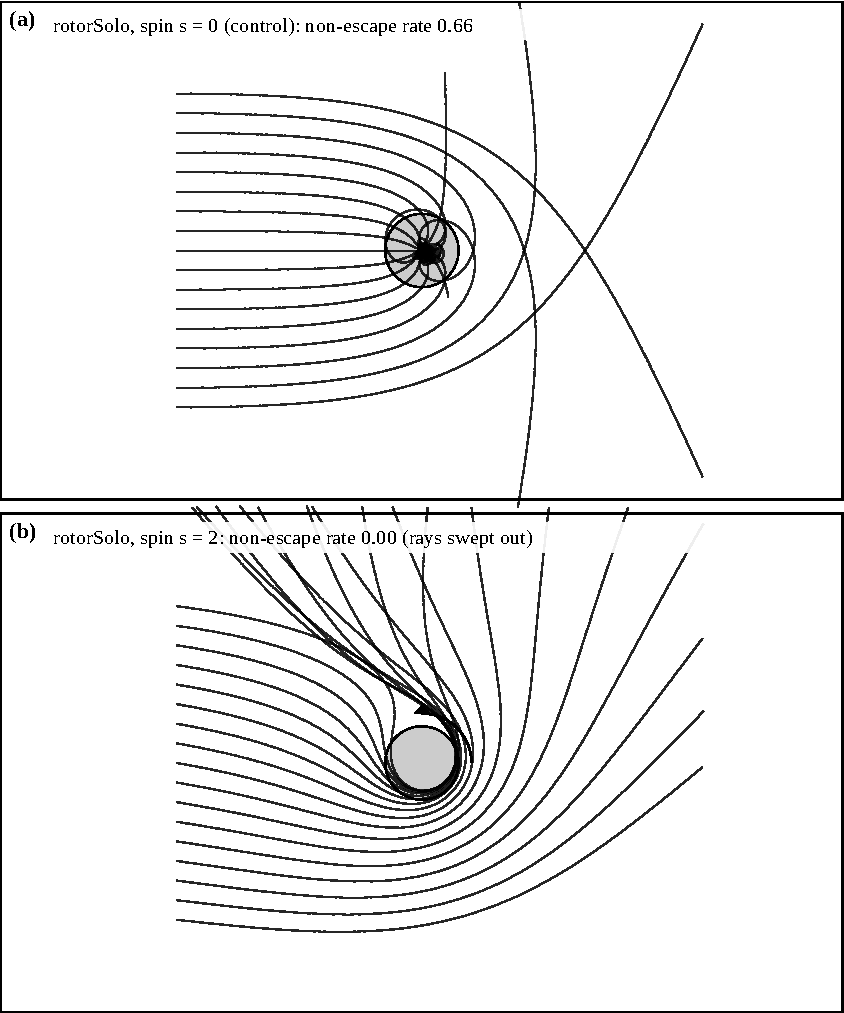
\includegraphics[width=\linewidth]{p2fig7.pdf}
  \caption{外来光線の掃き出し(プリセット \texttt{rotorSolo}。光線は $x=-300$ から $+x$ 方向へ
  刻み $2.7$ で $340$步進み、終端が $r=300$ の内側なら「非脱出」と数える---ゲート
  \texttt{behavior.rotorSolo} と同一の判定)。(a) スピン0の対照: 50本のファンの $62\%$ が
  捕捉される。(b) コアのスピン $s=2$(矢印は回転の向き): 捕捉は消え($0.00$)、ファンは
  非対称になる(平均最小接近半径は順行側 $158.2$ に対し逆行側 $72.4$)。自光チャネルは
  $s=0.3$ で既に飽和しているが、そのとき非脱出率はまだ $0.70$ である---2つの光学機構は
  独立である。物理対応ロック $\kappa=G/c^2=1/3600$ のもとでは $s=2$ でも掃き出しは起きない。}
  \label{fig:sweep}
\end{figure}

\subsection{満たされる要件と限界}

モデルの内側で、重く・高速スピンで・光学的に暗いコアは、
(i) $W$ の源となり重力し、(ii) 独立な2機構によって暗く、
(iii) 引きずりを通じて外縁回転曲線の増強に寄与する。半径分解プロファイルは
ブーストが内側に集中することを示す($v/v_{\mathrm{bar}}$ の増強は $r\approx121$ の
$1.58$ から $r\approx251$ の $1.16$ へ。8シード統計。図\ref{fig:curve})。したがってこの天体が\textbf{モデルの内側で}満たすのは、意図的に限定した
チェックリスト---自己発光の抑制・外来光線の除去・重力源であること・回転曲線への寄与---
であり、実在のダークマターに要求される現象論の全体(質量光度比・無衝突性・レンズ・
構造形成~\cite{BertoneHooper2018})には遠く及ばない。限界も同じ精度で
測られている: 逆設計問題(規定の外縁速度に合わせるパラメータ選択)は前方予測としては
正確(中央値残差 ${\approx}2\%$)だが、最外帯に届く前に方位角速度が飽和する。また
「引きずりだけが特定の銀河プリセットの腕を維持する」という以前の主張は、ノックアウト
検定が複合経路を示したときに撤回された。以上のどれも実在のダークマターについての
主張を許可しない(否定的主張4)。価値は、暗さについての要件水準の議論が、監査可能な
小さい系の中で明示的で反証可能なチェックリストになることである。
\begin{figure}[t]
  \centering
  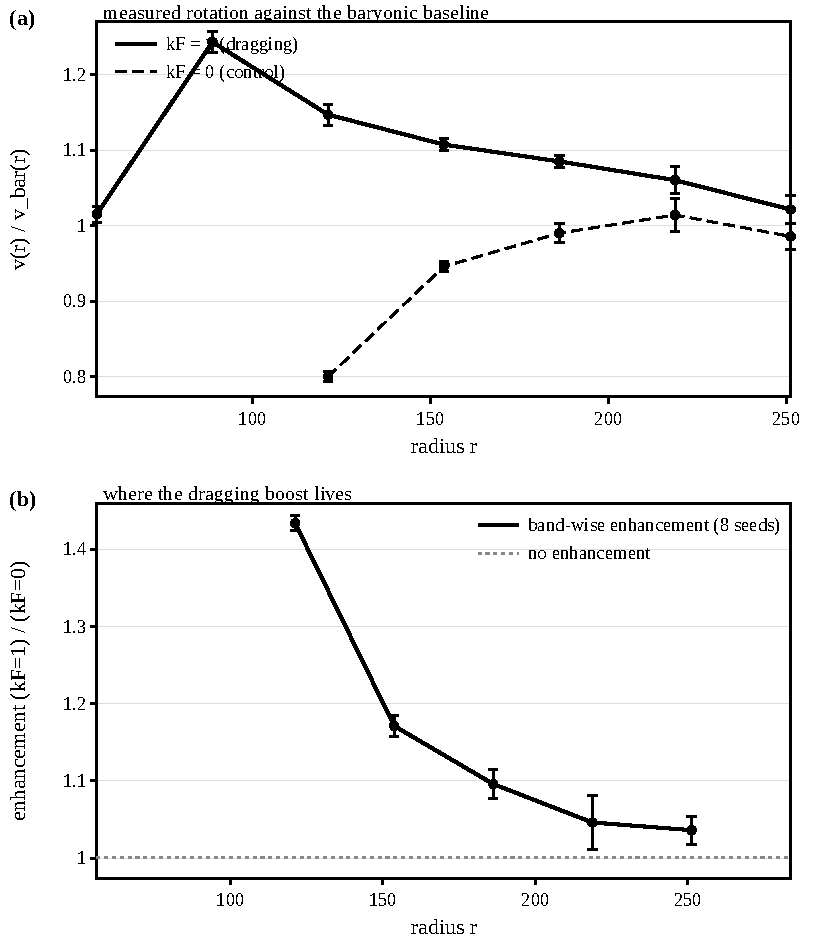
\includegraphics[width=\linewidth]{p2fig8.pdf}
  \caption{引きずりのブーストがどこにあるか(プリセット \texttt{galaxy}、8シード、$6000$步、
  $r\in[40,300]$ を8等分した帯。誤差棒はシード間の標準偏差 $\pm1$、粒子が3個未満になった
  帯はそのシードから除外)。(a) 実測 $v(r)$ と、実際の質量分布から計算したバリオン基準線
  $v_{\mathrm{bar}}(r)$ の比を、引きずりあり($k_F=1$)・なし($k_F=0$)で比較。
  (b) その2つの比、すなわち引きずりに帰せられる増強: $r\approx121$ の $1.58$ から
  $r\approx251$ の $1.16$ へ落ちる。ゲートの窓 $r\in[156,286]$ での帯平均外縁ブーストは、
  ここで使った beta 対象 build v1.41-b1 で $1.331\pm0.008$。\textbf{履歴}: 中間世代の
  エンジンで再生成した build v1.39-b1 では $1.074\pm0.006$($1.43\to1.04$ のプロファイル)
  だったが、変更履歴に記録されたエンジン巻き戻しにより現行値へ復帰し、第143便で図データ・
  キャプション・ゲートを再同期した。内側ほど強いという定性プロファイルは一貫して不変で
  ある。}
  \label{fig:curve}
\end{figure}

\begin{thebibliography}{99}
% 第143便: 論文1の実タイトル(dfm-paper.tex の \title)へ一致させた
% 第153便: 引用はアーカイブ済みレコードの実表題(主題のみ)に合わせる。
% 論文1の拡張副題は投稿時のレコード再登録で反映し、その時点で本 bibitem を更新
% (TODO(release) の範囲)。
\bibitem{DFM1} T. Imamura, \emph{Determinacy-Field Mechanics: A Machian Toy
Universe with Tunable Frame Dragging, Inverse-Square Gravity, and
Spin-as-Heat Analogies}, Zenodo (2026), doi:10.5281/zenodo.21454189.
% 第153便: 論文1に副題行が付いた(dfm-paper.tex \title)。DOI の指す
% Zenodo v1 レコードは主題のみを持つ。投稿時に再登録する。
\bibitem{Mach1893} E. Mach, \emph{The Science of Mechanics} (Open Court, 1893).
\bibitem{BarbourBertotti1982} J. B. Barbour and B. Bertotti, Proc. R. Soc. Lond. A \textbf{382}, 295 (1982).
\bibitem{Peacock1999} J. A. Peacock, \emph{Cosmological Physics} (Cambridge Univ. Press, 1999).
\bibitem{Leibundgut1996} B. Leibundgut \emph{et al.}, Astrophys. J. Lett. \textbf{466}, L21 (1996).
\bibitem{Goldhaber2001} G. Goldhaber \emph{et al.}, Astrophys. J. \textbf{558}, 359 (2001).
\bibitem{Fixsen2009} D. J. Fixsen, Astrophys. J. \textbf{707}, 916 (2009).
\bibitem{Noterdaeme2011} P. Noterdaeme \emph{et al.}, Astron. Astrophys. \textbf{526}, L7 (2011).
\bibitem{Planck2018} Planck Collaboration, Astron. Astrophys. \textbf{641}, A6 (2020).
\bibitem{Riess2022} A. G. Riess \emph{et al.}, Astrophys. J. Lett. \textbf{934}, L7 (2022).
\bibitem{Riess2024} A. G. Riess \emph{et al.}, Astrophys. J. \textbf{977}, 120 (2024).
% 第161便(P1-3): 既収載のこの項目がレビューの求めた2件目である(重複は追加しない)。
% TODO(ref-verify): 本環境では resolve できていない。投稿時に再確認する。
% 第161便(P1-3): 第VI節で引く JWST 期の距離梯子決定。
% TODO(ref-verify): 本環境は外部ネットワーク遮断のため arXiv 番号・掲載記録とも
% resolve できていない。投稿時に確認し、掲載版へ更新する。
\bibitem{Freedman2024} W. L. Freedman \emph{et al.}, arXiv:2408.06153 (2024).
\bibitem{DiValentino2021} E. Di Valentino \emph{et al.}, Class. Quantum Grav. \textbf{38}, 153001 (2021).
\bibitem{BertoneHooper2018} G. Bertone and D. Hooper, Rev. Mod. Phys. \textbf{90}, 045002 (2018).
\end{thebibliography}

\vspace{1em}
\noindent\textbf{訳注}: 本書は英語版 \texttt{dfm-paper2.tex} v0.9 の日本語訳である。
学術的な正本は英語版であり、相違がある場合は英語版が優先する。

\end{document}
